\documentclass[aspectratio=169]{beamer}
\usepackage{beamerthemetot}
\usepackage{graphicx}
\usepackage{animate}
\usepackage{calligra}
\usepackage[absolute,overlay]{textpos}
\usepackage[T1]{fontenc}
\usefonttheme{professionalfonts}
\usepackage{tikz}
\usetikzlibrary{shapes,arrows}
\usepackage{xcolor}
\usepackage{mathtools}
\usepackage{cancel}
 

\newcommand{\mytitle}{\color{White}\huge{\textbf{New Machine Learning Strategies for Data Scarce Material Science Problems}}}
\newcommand{\mysubtitle}{\color{Pink}\Large{\textbf{Go/No-go Meeting}}}
\newcommand{\myauthor}{\color{White}\textcalligra{\LARGE Ozgur Taylan Turan}}
\newcommand{\authorlabel}{\small O.T. Turan}
\author{\authorlabel}
\usepackage[backend=bibtex,firstinits=true,maxnames=30,maxcitenames=20,url=false,style=authoryear]{biblatex}

\setlength\bibitemsep{0.3cm} % space between entries in the reference list
\renewcommand{\bibfont}{\normalfont\scriptsize}
\renewcommand{\cite}[1]{\footnote<.->[frame]{\fullcite{#1}}}
\setbeamertemplate{bibliography item}{}
\bibliography{../../../archive_bib/library.bib}


\begin{document}

\setbeamercovered{transparent}

{
\def\beamer@entrycode{\vspace*{-\headheight}}
\setbeamertemplate{frametitle}[default][center]
\usebackgroundtemplate{\includegraphics[width=\paperwidth,height=\paperheight]{cover/coverart.pdf}}

\begin{frame}[plain] 

\begin{minipage}{\textwidth}
	\centering{\mytitle} \\
	\vspace{1cm}
	\centering{\color{White}\today} \\
	\vspace{1cm}
	\centering{\myauthor}\\
\end{minipage}


\end{frame}
}

\begin{frame}
  \centering
  \mysubtitle
\end{frame}

\begin{frame}{Outline}
  \centering
  \begin{itemize}
    \item Introduction 
    \item Literature
    \item Aim
    \item Research Questions
    \item Planning 
    \item Reflection 
  \end{itemize}
\end{frame}

%
% Meta Learning Definitions
Learning to learn, also referred to as meta-learning, treats the training of a machine learning model as a learning problem in itself. In the context of this work if a machine learning model's performance on a task is improving with training experiences it is said to be learning. In the light of this definition a machine learning model is said to be learning to learn if the performance on each task improves with training experience obtained from each task and with the number of tasks \cite{thrun1998}. Meta-learning recently is being used to tackle few-shot learning problems, where there is little data available from the learning task that is of prime interest, whereas there is an abundance of data from other similar tasks. 

% What Makes MAML Different
Early works of the learning-to-learn paradigm relied upon the one supervisory and one sub-ordinate model that interacts with each other for meta-learning. On one hand, sub-ordinate models try to improve the performance with training examples and on the other hand, the supervisory model tries to increase the performance over the family of tasks. MAML (Model-Agnostic Meta-Learning) \cite{finn2017} is a model that circumvents the need for supervisory and subordinate models. This method tries to tackle meta-learning by training any (As the name suggests MAML applies to all learners that improve performance by SGD (Stochastic Gradient Descent).) machine learning models parameters in a way to maximize the performance on a new learning task with few experiences through one or more gradient steps. 

% Where to use MAML?
MAML is used in few-shot learning problems in the supervised and reinforcement learning problems, where the losses differ from each other. Due to being model and problem independent MAML finds a wide application area in the context of few-shot meta-learning. Moreover, MAML also aims to improve a specific task performance quickly (with a few gradient steps). This is an additional aspect to our definition of meta-learning. 

% What is the problem?
As mentioned above, MAML aims to improve the generalization of a model for a certain learning task from a given family of tasks, with little data and minimal training. Minimal training indicates quick adaptation capabilities. This feature can prove useful in certain settings, for instance, in robotics research, where the reaction/adaptation time of the agents to dynamic environments bestow an inherent time limitation. However, this limitation is not present for the supervised learning problems, where MAML or its variants are utilized as a baseline. (\eg \cite{flennerhag2019, nichol2018, rajasegaran2020, collins2020, guiroy2019} etc.) Most of the unsupervised problem benchmark is image detection problem, where $N$-way $K$-shot classification problem ($N$ different classes with $K$ labeled training data) is tried to be tackled. Given the nature of the problem, most of the time memory or time limitation does not constitute a major issue in the given problem setting.

% What is our paper about?
The main aim of this paper is to investigate the MAML under the settings where quick adaptation is not needed, and where most of the applications and variants of this method are benchmarked. This will be achieved by looking at the expected performance of the MAML under 2 regression scenarios, and comparing its performance to conventional base learners (\eg Linear Regression, Ridge Regression, Kernel Ridge Regression, etc.). By doing this we aim to investigate the effect of the limited adaptation step.% In the meantime, the effect of task variance, and noisy observations (unlike the setting presented in \cite{finn2017}) will also be investigated.



\section{Introduction}
\begin{frame}{Computational Solid Mechanics}
  \begin{minipage}{0.5\textwidth}
    \only<1>{
    \begin{block}{\color{White} Solid Mechanics}
      \begin{itemize}
        \item \color{Black} Relate deformation with internal force development
        \item $\boldsymbol{\nabla} \cdot \mathbf{P}= 0$ with \color{White} $\mathbf{P}=\mathcal{C}(\mathbf{F})$
      \end{itemize}
    \end{block}
    }
    \only<2>{
    \centering
    \includegraphics[width=0.85\textwidth]{Figures/intro/link}
    }
  \end{minipage}%
  \begin{minipage}{0.5\textwidth}
    \only<1>{
    \centering
    \includegraphics[width=0.85\textwidth]{Figures/intro/link}
    }
    \only<2>{
    \begin{block}{\color{White}Finite Element Method}
      \begin{itemize}
        \item General PDE solving method
        \item Discretize the domain 
        \item Weakly satisfy the PDE at selected points
      \end{itemize}
    \end{block}
  }
  \end{minipage}
\end{frame}

\begin{frame}{Composite Modeling}
  \begin{minipage}{0.5\textwidth}
  \only<1>{
    \centering
    \includegraphics[width=2\textwidth]{Figures/intro/scales}
    }
    \only<2>{
    \begin{block}{\color{White}FE$^2$}
      \begin{itemize}
        \item Representative Volume Element (RVE)
        \item Solve for RVE and average the response
        \item Repeat for every selected point
      \end{itemize}
    \end{block}
  }

  \only<3,4>{
  \begin{block}{\color{White}FE$^2$-Bottleneck}
      \begin{itemize}
        \item Micro-scale problem solution
        \item Repeating for every selected point
        \item Highly non-linear behaviour 
      \end{itemize}
    \end{block}
  }
  \end{minipage}%
  \begin{minipage}{0.5\textwidth}
  \only<2>{
    \centering
    \includegraphics[width=0.9\textwidth]{Figures/intro/FE2-CONV}
  }
  \only<3,4>{
    \centering
    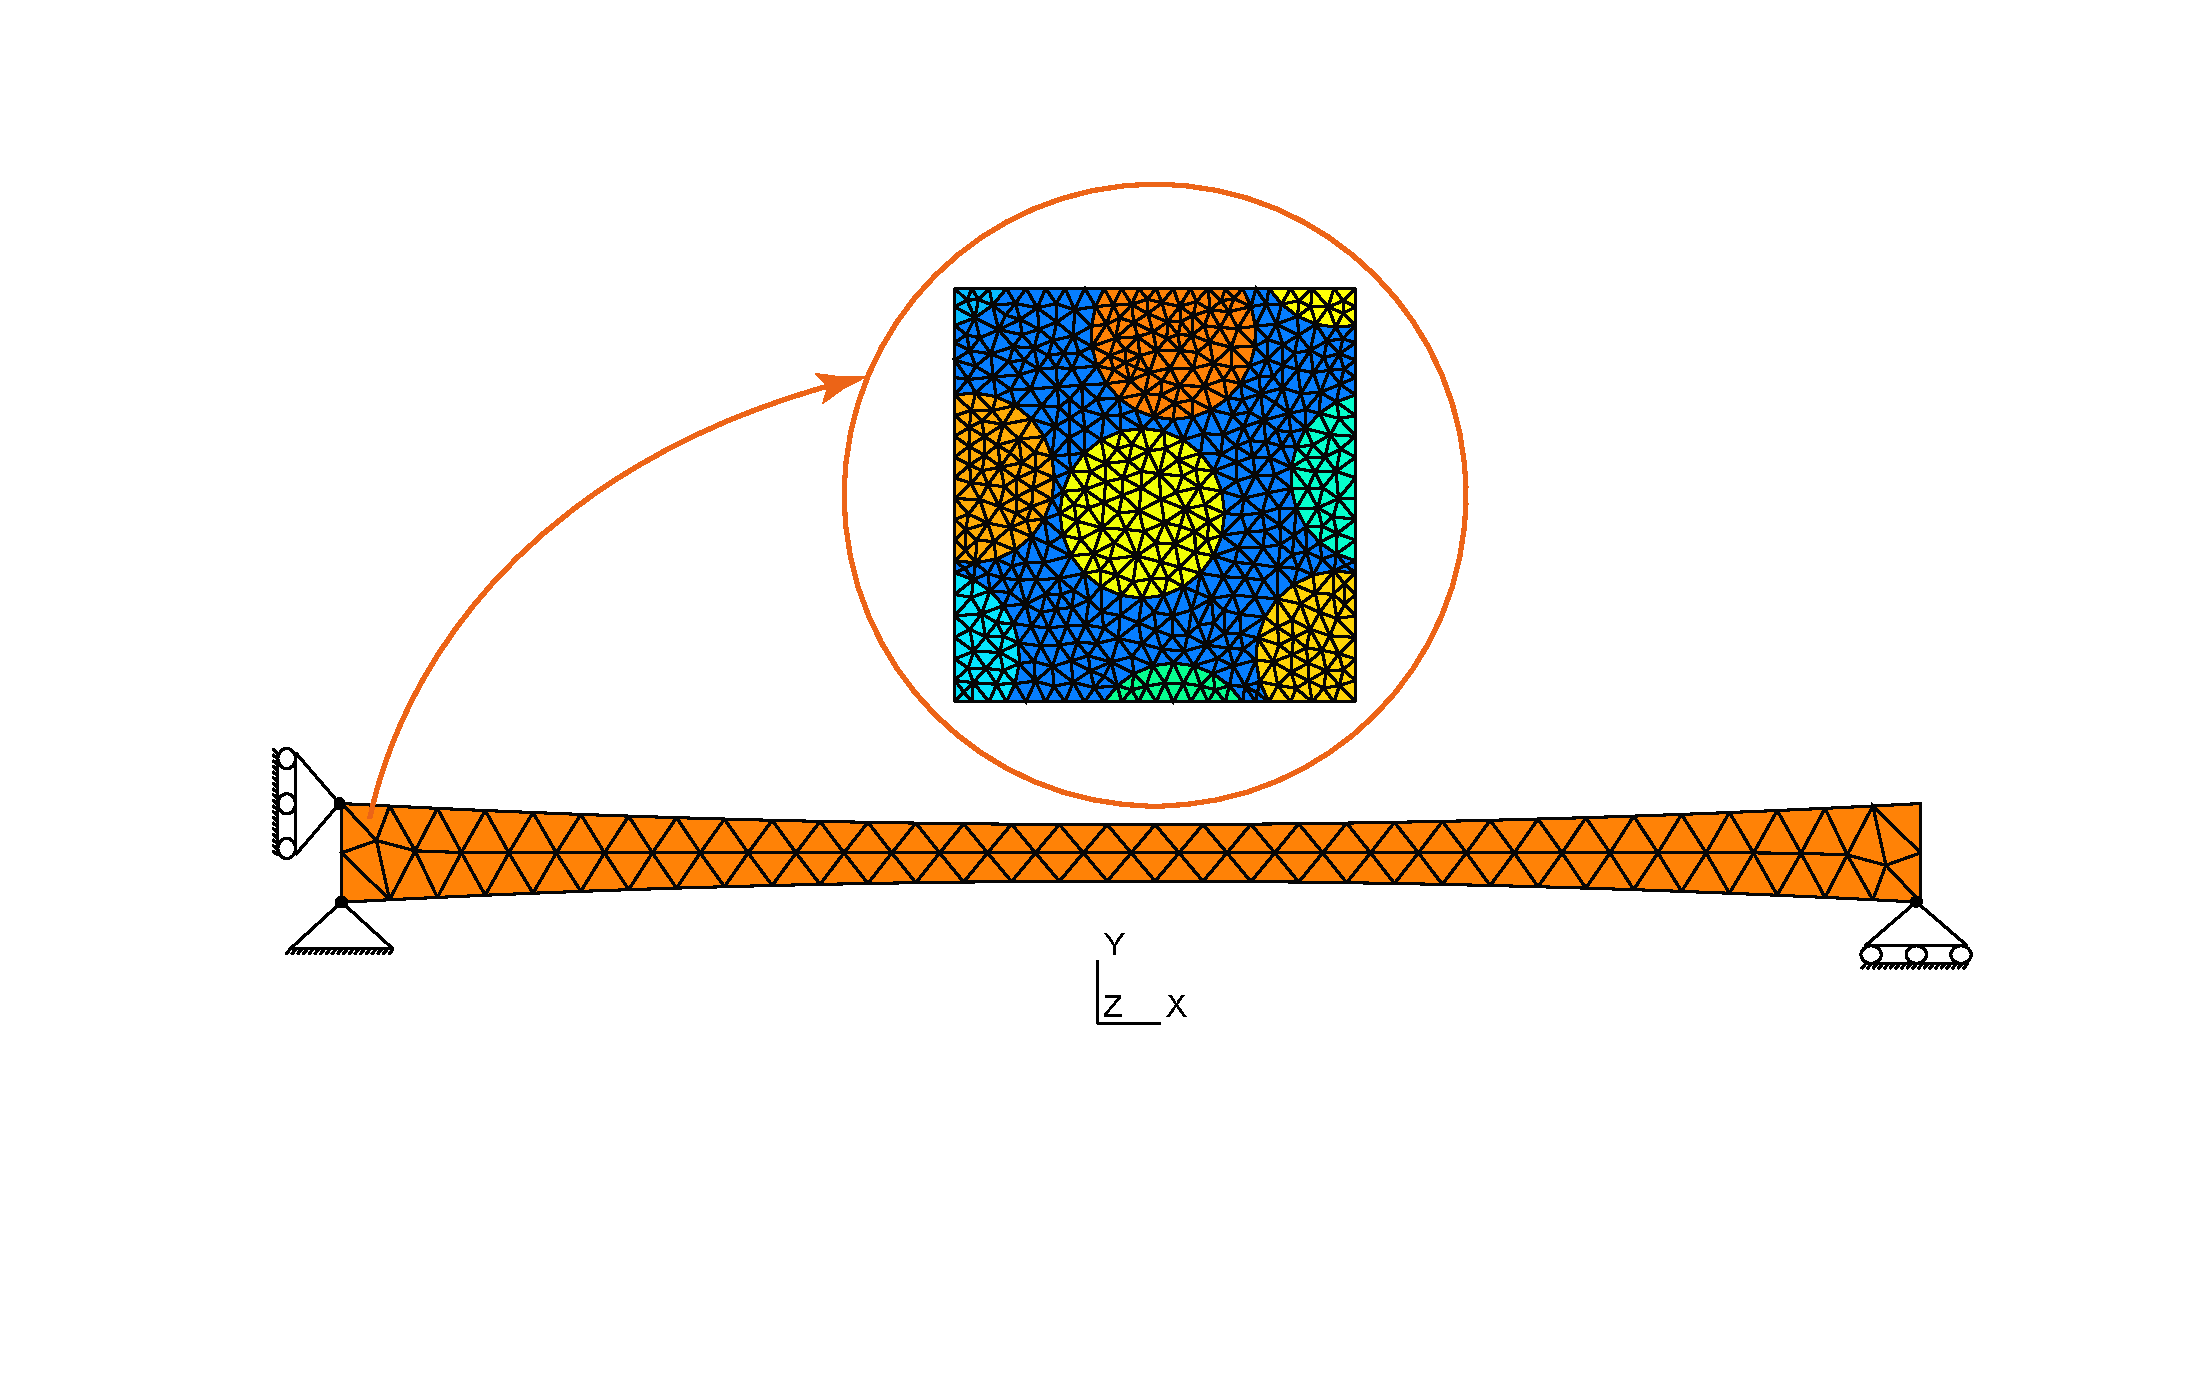
\includegraphics[width=\textwidth]{Figures/intro/bone}
  }
  \end{minipage}
  \only<4>{
    \centering
    \color{Pink} We need multiple of these simulations for real world applications!
  }
\end{frame}


\section{Literature}

\begin{frame}{FE$^2$ via Machine Learning}
  \begin{minipage}{0.5\textwidth}
  \only<1-2>
  {
    \centering
    \includegraphics[width=0.9\textwidth]{Figures/intro/FE2-CONV}
  }
  \only<3>
  {
    \begin{block}{\color{White} Problems in Current State}
      \begin{itemize}
        \item Risky Extrapolation
        \item Data Scarcity
        \item Single Parameter Configuration
        \item General Applicability
      \end{itemize}
    \end{block}
  
  }
  \end{minipage}%
  \begin{minipage}{0.5\textwidth}
  \only<1-3>
  {
    \centering
    \includegraphics[width=0.9\textwidth]{Figures/literature/FE2-ML}
  }
  \end{minipage}
\only<2>
{
  \begin{itemize}
  \centering
    \item \color{Pink} Computationally a Material: $\mathbf{F} \to \mathbf{P}$
  \end{itemize}
}
\end{frame}

\begin{frame}{Hypothesis}
  \begin{itemize} 
    \item Most of the problems encountered can be tackled with more general approaches.
    \item The core problem is finding the mapping between a deformation measure and a force measure. ($\mathbf{P}=\mathcal{C}(\mathbf{F})$).
    \item Similarity between the problems can be exploited, without considering the different parameters that effect the model.
  \end{itemize}
\end{frame}







\section{Aim}

\begin{frame}{Aim-\only<1>{A}\only<2>{B}}
\only<1>{
  \begin{minipage}{0.5\textwidth} 
    \includegraphics[width=\textwidth]{Figures/literature/FE2-ML.pdf}
  \end{minipage}%
  \begin{minipage}{0.5\textwidth} 
    \includegraphics[width=\textwidth]{Figures/problem/models.pdf}
  \end{minipage}
}
\only<2>
{
  \begin{minipage}{0.3\textwidth} 
    \centering
    \includegraphics[width=\textwidth]{Figures/problem/collective.pdf}
  \end{minipage}%
  \begin{minipage}{0.7\textwidth} 
    \centering
    \includegraphics[width=\textwidth]{Figures/problem/material.pdf}
  \end{minipage}
}
\end{frame}

\begin{frame}{Overall Learning Problem-\only<1>{A}\only<2>{B}}
  \only<1>
{
  \color{Pink} Consider an arbitrary space that represents overall material behaviour, and the subsets of this space representing specific material types.
  \centering
  \includegraphics[width=0.6\textwidth]{Figures/problem/tasks}
}
  \only<2>
{
  \centering
  \includegraphics[width=0.5\textwidth]{Figures/problem/tasks_example}

  \begin{itemize}
  \item \color{Pink} Every label in this space becomes a full mapping! ( $T_{D_1}:=\{T_{{D_1}_i}:\mathbf{F}\to\mathbf{P}_i\}_{i=1}^M$)
  \end{itemize}
}
\end{frame}



\section{Research Questions}
\begin{frame}{Research Questions}
  %\color{Pink} Prediction of a mapping $\mathcal{T}_{\mathcal{A}^\prime}$ given a batch of mappings $\{\mathcal{T}_{\mathcal{A}_i}\}_{i=1}^{M}$ where $\mathcal{A}^\prime \in \boldsymbol{\mathcal{A}}$
  \begin{itemize}
    \item To what extent this prediction is possible?
    \item Can we find a latent space where the tasks with different parameters live and exploit the similarities between these tasks?
    \item What information can we extract from the model trained with the batch of tasks at hand?
    \item Can we find an effective sampling strategy in the task space and in the feature space of the given task?
  \end{itemize}
\end{frame}

\begin{frame}{Related Paradigms in ML Literature}
  \begin{itemize}
    \centering
    \item \color{Pink} Meta Learning (Learning-to-learn) \color{Black}
    \item Transfer Learning and Domain Adaptation
    \item Multi-task Learning
  \end{itemize}
\end{frame}


\section{Planning}

\begin{frame}{Project Planning}
  \includegraphics[width=0.85\textwidth]{Figures/planning/project_plan}
\end{frame}

\begin{frame}{Collaborations}
  \begin{itemize}
    \item Continuation of my MSc. Thesis Multi-fidelity Gaussian Process Regression 
    \item Miguel Bessa and I in collaboration with Iuri Rocha and Frans van der Meer from Civil Engineering and Geosciences  
    \item Data Generation
  \end{itemize}
\end{frame}

\begin{frame}{Doctoral Education Planning}
\centering
  \includegraphics[width=0.8\textwidth]{Figures/planning/doctoral_education_plan}
\end{frame}



\section{Reflection}
\begin{frame}{Past Year with COVID19}
  \begin{minipage}{0.45\textwidth}
    \begin{block}{\color{White} Academic}
      \begin{itemize}
        \item PRB 
        \item Collaboration
      \end{itemize}
    \end{block}
  \end{minipage}%
  \hspace{5mm}
  \begin{minipage}{0.45\textwidth}
    \only<2>
    {
    \begin{block}{\color{White} Non-Academic}
      \begin{itemize}
        \item Work-Life Balance
        \item Well-being
      \end{itemize}
    \end{block}
  }
  \end{minipage}
\end{frame}

\begin{frame}
  \centering
  \color{Pink} Thanks for your attention!
\end{frame}
\section{Extras}
\begin{frame}{Reformulate the Problem-\only<1>{A}\only<2>{B}}
  \begin{minipage}{0.5\textwidth}
\only<1>
{
    \begin{block}{\color{White} $\mathbf{P}=\mathcal{C}(\mathbf{F})$}
      \begin{itemize}
        \item Normally, $\mathbf{P}=f(\mathbf{F}, \boldsymbol\gamma)$
        \item $\boldsymbol{\gamma}:=\{\gamma_i\}_{i=1}^{M}$ with $M\in\mathbb{Z}^+$
        \item $\mathbf{P}=\mathcal{M}(\mathbf{F}, \boldsymbol{\gamma})$
        \item Application specific models! 
      \end{itemize}
    \end{block} 
}
\only<2>
{
    \begin{block}{\color{White} $\mathbf{P}=\mathcal{C}(\mathbf{F})$}
      \begin{itemize}
        \item Let's stick to $\mathbf{P}=\mathcal{C}(\mathbf{F})$
        \item Then, $\mathbf{P}=\mathcal{M}(\mathbf{F})$
      \end{itemize}
    \end{block} 
    \begin{block}{\color{White} How to account for $\boldsymbol{\gamma}$?}
      \begin{itemize}
        \item Let's stick to $\{\mathbf{P}_i=\mathcal{C}_i(\mathbf{F})\}_{i=1}^{M}$ with $M\in\mathbb{Z}^+$
        \item $\mathbf{P}=\mathcal{M}(\mathbf{F})$
        \item Model input-output remains the same!
      \end{itemize}
    \end{block} 
}
  \end{minipage}%
  \begin{minipage}{0.5\textwidth}
    \centering
    \includegraphics[width=0.9\textwidth]{Figures/literature/FE2-ML.pdf} 
  \end{minipage}
\end{frame}

\begin{frame}{Reformulate the Problem-\only<1>{C}\only<2>{D}}
  \begin{minipage}{0.5\textwidth}
\only<1>
{
    \begin{block}{\color{White} How do we end up with a parametrized relationships?}
      \begin{itemize}
        \item Series of assumptions, $\mathcal{A}:\{a_n \subset a_{n-1} \subset ... \subset a_1\}$ 
     \end{itemize}
    \end{block} 
    \begin{block}{\color{White} Individual Learning Problem}
      \begin{itemize}
        \item If the aim is to learn $\mathbf{F} \to \mathbf{P}$ 
        \item Learning problem: $\mathcal{T}_\mathcal{A}:\mathbf{F} \to \mathbf{P}$
      \end{itemize}
    \end{block}
}
\only<2>
{
    \begin{block}{\color{White} Overall Learning Problem}
      \begin{itemize}
        \item Given $\{\mathbf{P}_i=\mathcal{C}_i(\mathbf{F})\}_{i=1}^{M}$ with $M\in\mathbb{Z}^+$
        \item Learning problem: $\{\mathcal{T}_{\mathcal{A}_i}:\mathbf{F} \to \mathbf{P}_i\}_{i=1}^{M}$
      \end{itemize}
    \end{block} 
}
  \end{minipage}%
  \begin{minipage}{0.5\textwidth}
    \centering
    \includegraphics[width=0.9\textwidth]{Figures/literature/FE2-ML.pdf} 
  \end{minipage}
\end{frame}

\begin{frame}{Single-Task Learning vs Bias Learning-\only<1>{A}\only<2>{B}}
  \only<1>
  {
    \begin{block}{\color{White} Single-Task Learning}
      \begin{itemize}
        \item Input Space $\mathbf{F}$ OutputSpace $\mathbf{P}$
        \item Probability Distribution $p$ on $\mathbf{F}\times\mathbf{P}$
        \item Loss Function $l:\mathbf{P}\times\mathbf{P}\to \mathbb{R}$
        \item Hypothesis Space $\mathcal{H}$, a set of functions $h:\mathbf{F}\to\mathbf{P}$
        \item Minimize the expected loss to get $h\in\mathcal{H}$
      \end{itemize}
    \end{block}
  }
  \only<2>
  {
    \begin{block}{\color{White} Bias  Learning}
      \begin{itemize}
         \item Input Space $\mathbf{F}$ OutputSpace $\mathbf{P}$
        \item Probability Distribution $p$ on $\mathbf{F}\times\mathbf{P}$
        \item Loss Function $l:\mathbf{P}\times\mathbf{P}\to \mathbb{R}$
        \item An environment $(\mathcal{Q},\mathcal{P})$ where $\mathcal{P}$ is all possible distribution of $p$ and $\mathcal{Q}$ is the distribution of $\mathcal{P}$
        \item Hypothesis Space Family $\mathbb{H}:=\{\mathcal{H}\}$, where each $\mathcal{H}$ is a set of functions $h:\mathbf{F}\to\mathbf{P}$
        \item Minimize the expected future risk or transfer risk to find the appropriate Hypothesis Space $\mathcal{H}$ 
      \end{itemize}
    \end{block}
  }
\end{frame}

\begin{frame}{MAML vs Multi-task}
	\begin{itemize}
		\item Problem: $y=a*\text{sin}(x+p)$ for $x\in[0,5]$ and $a\in[0.1,5]$ \& $a\in[0,\pi]$ for $\text{K}=5$ and $\mathcal{B}(\mathcal{T})$ size $100$
	\end{itemize}
	\begin{minipage}{0.5\textwidth}
		\includegraphics[width=0.9\textwidth]{Figures/Study1/sine-hard-finn-maml-pred.pdf}
		\centering
			MAML
	\end{minipage}%
	\begin{minipage}{0.5\textwidth}
		\includegraphics[width=0.9\textwidth]{Figures/Study1/sine-hard-finn-multitask-pred.pdf}
		\centering
			Multi-task
	\end{minipage}
\end{frame}

\begin{frame}{Small Investigation of MAML \cite{Finn2017}}
  \begin{minipage}{0.5\textwidth}
    \begin{itemize}
      \item $ a \in \mathbb{R}^d \to p_a \sim \mathcal{N}(m\mathbf{1},c\mathbf{I})$
      \item $ x \in \mathbb{R}^d \to p_x \sim \mathcal{U}(\mathbf{0},b\mathbf{1})$
      \item $ \varepsilon \sim \mathcal{N}(0,\sigma^2)$
      \item $ y = a^\text{T}x + \varepsilon \quad \in \mathbb{R}$
      \item $ Z:= ((x_i,y_i))_{i=1}^N$
      \item $ \hat{a}_N \to $ an estimator trained with N training points
    \end{itemize}
  \end{minipage}%
  \begin{minipage}{0.5\textwidth}
    Expected Error over the whole task space,
      $ \int \int \int (\hat{a}_N(Z)^{\text{T}}x-y)^2p(x,y)dxdyp_ZdZp_ada$
  \end{minipage}
  \color{Pink} Investigating the performance of a future emprical risk minimizing algorithm for transfer risk.
\end{frame}

\begin{frame}{F3DASM}
\centering
\begin{minipage}{0.55\textwidth}
		\begin{itemize}
		\item Design of Experiements
		\item Simulation or Machine Learning Module
	\end{itemize}	
\end{minipage}

\begin{minipage}{0.4\textwidth}
	\includegraphics[width=\textwidth]{Figures/F3DASM/doe}
\end{minipage}%
\hspace{1mm}$\xRightarrow{\text{FEM}(\mathbf{F})}$
\begin{minipage}{0.4\textwidth}
	\includegraphics[width=\textwidth]{Figures/F3DASM/manifold}
\end{minipage}%
\end{frame}

\begin{frame}{Summer Schools \& Conferences}
\only<1>
{
  \begin{block}{\color{White} Summer Schools}
  \begin{itemize}
    \item Machine Learning Summer Schools (MLSS)
    \item Gaussian Process Summer School 
    \item Nordic Probabilistic AI Summer School
    \item Oxford Machine Learning Summer School
  \end{itemize}
  \end{block}
}
\only<2>
{
  \begin{block}{\color{White} Conferences on ML}
  \begin{itemize}
    \item Conference on Computer Vision and Pattern Recognition (CVPR)
    \item International Conference on Learning Representations (ICLR)
    \item International Conference on Machine Learning (ICML)
    \item International Conference on Machine Learning and Pattern Recognition (ICMLPR)
  \end{itemize}
  \end{block}
}

\only<3>
{
  \begin{block}{\color{White} Conferences on Mechanics}
  \begin{itemize}
    \item FEniCS Conference
    \item International Conference on Mathematics and Computational Mechanics (ICMCM)
    \item International Conference on Computational Geomechanics and Material Response (ICCGMR)
    \item FEniCS Conference
    \item International Conference on Computational Continuum Mechanics and Dynamics (ICCCMD)
\item International Conference on Computational Continuum and Continuum Mechanics (ICCCM)
  \end{itemize}
  \end{block}
}
\end{frame}





\end{document}
